\documentclass[12pt]{article}
\usepackage[utf8]{inputenc}
\usepackage{hyperref}
\usepackage{tikz}
\usetikzlibrary{positioning}
\usepackage{caption}
\usepackage{amsmath}
\usepackage[margin=1in]{geometry}
\usepackage{graphicx}
\usepackage[linesnumbered,ruled,vlined]{algorithm2e}

\title{Search Problems}
\author{Shaan Fulton}
\date{\today}

\begin{document}

\maketitle

Many problems can be understood as search problems. A search problem is any problem which involves a:

\begin{itemize}
	\item Set of possible states
	\item A start state
	\item A goal state
	\item A successor function (a function which returns what states can be achieved from a given state)
\end{itemize}

In other words, it's a problem where we must determine a set of actions (that fall within our successor function) to achieve our goal state from our start state.

\section*{Pathfinding as a Search Problem}

\subsection*{1. Set of Possible States}

Each state is a position on a grid. Here is the full set of states for a 3x3 grid:

\begin{center}
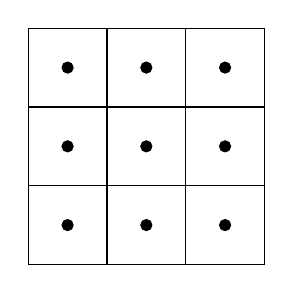
\begin{tikzpicture}
    \foreach \x in {0,1,2} {
        \foreach \y in {0,1,2} {
            \draw (\x, \y) rectangle ++(1,1);
            \filldraw[black] (\x+0.5, \y+0.5) circle (2pt);
        }
    }
\end{tikzpicture}
\end{center}

This represents 9 possible states (positions), arranged in a 3x3 grid.

\subsection*{2. Start State}

\begin{center}
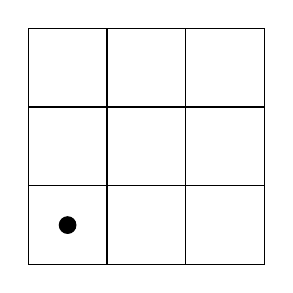
\begin{tikzpicture}
    \foreach \x in {0,1,2} {
        \foreach \y in {0,1,2} {
            \draw (\x, \y) rectangle ++(1,1);
        }
    }
    % Character at (0,0)
    \filldraw[black] (0.5, 0.5) circle (3pt);
\end{tikzpicture}
\captionof{figure}{Start state: character begins in the bottom-left corner}
\end{center}

\subsection*{3. Goal State}

\begin{center}
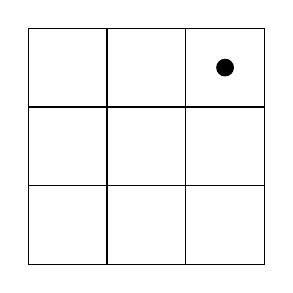
\begin{tikzpicture}
    \foreach \x in {0,1,2} {
        \foreach \y in {0,1,2} {
            \draw (\x, \y) rectangle ++(1,1);
        }
    }
    % Character at (2,2)
    \filldraw[black] (2.5, 2.5) circle (3pt);
\end{tikzpicture}
\captionof{figure}{Goal state: character must reach the top-right corner}
\end{center}

\subsection*{4. Successor Function}

From any given position, the character can move one square up, down, left, or right (if within bounds). For example, from the center of the grid:

\begin{center}
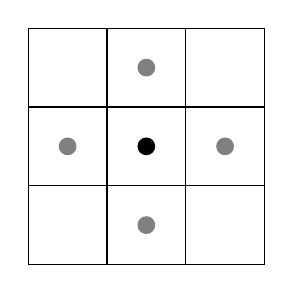
\begin{tikzpicture}
    % Draw the grid
    \foreach \x in {0,1,2} {
        \foreach \y in {0,1,2} {
            \draw (\x, \y) rectangle ++(1,1);
        }
    }
    % Main character at center
    \filldraw[black] (1.5, 1.5) circle (3pt);
    % Gray potential successors
    \filldraw[gray] (0.5, 1.5) circle (3pt); % left
    \filldraw[gray] (2.5, 1.5) circle (3pt); % right
    \filldraw[gray] (1.5, 0.5) circle (3pt); % down
    \filldraw[gray] (1.5, 2.5) circle (3pt); % up
\end{tikzpicture}
\end{center}

From the center, the successor function returns:
\begin{itemize}
    \item Move up: (1,2)
    \item Move down: (1,0)
    \item Move left: (0,1)
    \item Move right: (2,1)
\end{itemize}

\bigskip

Thus, the problem of pathfinding — determining how to move from the start state to the goal state — is clearly a search problem. However, search problems extend beyond pathfinding. The Tower of Hanoi is a famous example.

\begin{figure}[h]
  \centering
  \includegraphics[width=0.5\textwidth]{general-search-hanoi.jpg}
	\caption{A Tower of Hanoi, Solved}
  \label{fig:tower}
\end{figure}

\newpage

\section*{General Tree Search Strategies}

Many search problems can be understood in terms of decision trees. We imagine the nodes in the decision tree form the decisions we make along a path we are constructing. The branches from a node represent the results of the successor function applied to that node. The tree is a useful although not necessary model for many search problems, especially those in which looping is not desired.

But how do we traverse these decision trees? Let's suppose we have the following decision tree:

\vspace{2em}
\begin{center}

\begin{tikzpicture}[
  node distance=2cm and 3cm,
  every node/.style={draw=none, inner sep=0pt}
]

% Root node (dot at (0,0))
\node (start) {
  \begin{tikzpicture}[scale=0.6]
    \foreach \x in {0,1,2} {
      \foreach \y in {0,1,2} {
        \draw (\x, \y) rectangle ++(1,1);
      }
    }
    \filldraw[black] (0.5,0.5) circle (3pt); % dot at (0,0)
  \end{tikzpicture}
};

% Left child: move right (dot at (1,0))
\node[below left=of start] (right) {
  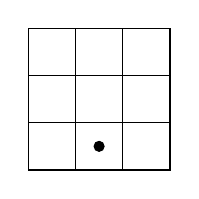
\begin{tikzpicture}[scale=0.6]
    \foreach \x in {0,1,2} {
      \foreach \y in {0,1,2} {
        \draw (\x, \y) rectangle ++(1,1);
      }
    }
    \filldraw[black] (1.5,0.5) circle (3pt); % dot at (1,0)
  \end{tikzpicture}
};

% Right child: move up (dot at (0,1))
\node[below right=of start] (up) {
  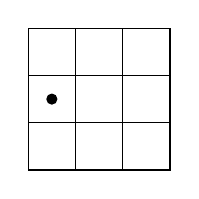
\begin{tikzpicture}[scale=0.6]
    \foreach \x in {0,1,2} {
      \foreach \y in {0,1,2} {
        \draw (\x, \y) rectangle ++(1,1);
      }
    }
    \filldraw[black] (0.5,1.5) circle (3pt); % dot at (0,1)
  \end{tikzpicture}
};

% Draw edges
\draw[-latex, thick] (start) -- (right);
\draw[-latex, thick] (start) -- (up);

\end{tikzpicture}


\end{center}

If we suppose our goal to be in the top right corner, which successor should we choose?

This all depends on the search strategy we employ. The search strategy simply tells us of all the successors which one we should choose next. We consider the following:

\begin{itemize}
	\item Depth-first search. This searches the ``left-most" successor recursively. This means it quickly descends the search tree.
	\item Breadth-first search. This searches every successor of a given node, or every node in a tree layer, before moving on to the next. To gradually descends but investigates all options as it goes.
	\item Uniform cost search. This searches successors according to cost prioritization: it will always select the next cheapest option available.
	\item A* search. This queues up and selects the next cheapest and hueristically advantageous option. That is, we create some hueristic (like linear distance to goal) and build this into our successor prioritization.
\end{itemize}

Interestingly, every search strategy is implemented in effectively the same way:

\begin{itemize}
	\item Construct a queue, or ``fringe", representing the states we will explore next in order. Add your initial state to the queue.
	\item Pick the first item off the queue and check if it is the goal state. If so, return your path. If not, continue.
	\item If not on a goal state, run your successor function to determine what your next options are. Add these options to the queue according to your strategy.
	\item Repeat, picking the next state off your queue.
\end{itemize}

In these implementations, we'll often pass path and state together so that when we return, we can return not only that we have discovered a goal state, but also the relevant path to get us there.

In psuedocode:

\vspace{2em}

\begin{algorithm}[H]
\caption{Generic Search Algorithm}
Initialize the \textbf{fringe} with the initial state and path\;
\While{fringe is not empty}{
    Remove the first element from the fringe: \texttt{(current\_state, path)}\;
    \If{current\_state is a goal state}{
        \Return path\;
    }
    \ForEach{successor of current\_state}{
        Add (successor, path + successor) to the fringe according to your strategy\;
    }
}
\end{algorithm}

\vspace{2em}

We will evaluate each strategy below. Note that we can evaluate these algorithms according to 4 key factors:

\begin{itemize}
	\item Complete - is it guaranteed to provide a solution?
	\item Optimal - is it guaranteed to find the least cost path?
	\item What is it's time complexity?
	\item What is it's space complexity?
\end{itemize} 

\subsection*{Depth First Search}

The idea behind DFS is simple. Go deep. When constructing our fringe, the deepest node takes priority. That is, the node most far down the search tree. This is easily programmed in: just use a stack, as a stack is first in, last out, so the newest successors to be added will be prioritized, rather than those "higher up" successors added early on (which we will forget about unless we reach the bottom of our options without finding a goal and must backtrack.

DFS is complete. It will eventually exhaust all options and thus will find a solution if it exists.

DFS is not optimal, however. It will happily output an extremely long and costly path. It doesn't consider path length or cost - in fact, it's geared towards sending a longer path as it will happily explore down one, very, very long search tree to get to a goal.

DFS time complexity is often terrible as it is choosing the next successor in a sort of random fashion. There is no heuristic to guide it.

\subsection*{Breadth First Search}

BFS explores every option at a particular depth (or every successor from one state) before continuing down the tree to the successor of those successors. This is programmed in with a queue, and is therefore first in first out (the earliest to be added will leave first).

BFS is complete. It will eventually exhaust all options.

BFS is optimal in path length but not necessarily in cost. It does not account for cost. However, it will find the shortest path from our initial state to our goal state, as every option at each distance level is explore before moving on to another distance level.

BFS can have high time complexity as it does not rely on a heuristic and will happily explore all options if your goal is far enough away. This is especially problematic if your goal is always expected to be very deep. This is often the case for constraint specification problems (CSPs—see \texttt{constraint-specification}) making BFS algorithms particularly slow for these problem types.

\subsection*{Uniform Cost Search}

Uniform Cost Search simply identifies the next successor based on \textbf{total cost}. This is only applicable if different successors carry different costs of ``travel." To program this, we create a ``priority queue," in which lower cost options are prioritized. The total cost distinction is important: the priority is based on the total cost to get to a given node. Therefore, nodes placed in queue earlier will get picked up even if they're quite expensive, as eventually the cost of going down one path will outweight the cost of making the leap to an expensive choice.

UCS is complete. it too will eventually exhaust all options.

UCS is cost and path distance optimal.

\subsection*{A* Search}

A* (A-star) search relies on a priority queue like UCS. However, it prioritizes the next option not solely based on cost, but also based on a heuristic of our choice. This heuristic helps point the algorithm in the right direction. For instance, it may be the linear distance from our state to the goal. This can be very powerful, as we are no longer spending time exploring fruitless paths. For instance, in a mapping algorithm, imagine if we searched for our destination by extending out in all directions! With A-star, we only head our search in an appropriate direction.

A-start is very dependent on the heuristic. We explore A* heuristics and their classifications in \texttt{a-star-heuristics}.


\end{document}

